\setchapterpreamble[u]{\margintoc}
\chapter{Electrodinámica cuántica}
\labch{Part}

\begin{center}
  \large Todo esto lo he sacado del \cite{Dobdado}
\end{center}
La electrodinámica cuántica (QED) describe la interacción entre electrones (o cualquier otra partícula cargada de spin $1 / 2$ como los muones, quarks, etc) y los fotones, así como las interacciones de las partículas cargadas entre sí. La teoría fue desarrollada por F. Dyson, R. Feynman, J. Schwinger y S. Tomonaga a finales de los años 40 y es la primera teoría cuántica de campos que permitió hacer cálculos de forma consistente. La constante de acoplo de la teoría viene dada por la carga del electrón $e$, o más concretamente, por la constante de estructura fina $\alpha=e^{2} / 4 \pi \hbar c \simeq 1 / 137$ que es una cantidad pequeña y por tanto la teoría permite un desarrollo perturbativo como el que hemos visto en el tema anterior.

En este tema estudiaremos las reglas de Feynman para QED y los principales procesos de interacción.
\section{Lagrangiano clásico e invariancia Gauge}
\section{Cuantización, teoría de perturbaciones y reglas de Feymann}
\section{Reglas de Feynman}
\subsection{Alguna fórmulas útiles}
\begin{equation}
  \begin{array}{ll}
  g_\mu^\mu=4=\delta_\mu^\mu & \gamma^0=\gamma^{0^ \dagger} \\
  \left\{\gamma^\mu, \gamma^\nu\right\}=2 g^{\mu \nu} & \gamma^i=-\gamma^{i ^\dagger} \\
  \gamma_\nu \gamma^\mu \gamma^\nu=-2 \gamma^\mu & \left(\gamma^0\right)^2=1 \\
  \gamma_{\mu}=g_{\mu\nu} \gamma^\nu &\gamma^{\mu^\dagger}=\gamma^\sigma \gamma^\mu \gamma^\sigma \\
  \gamma^\rho \gamma^\mu \gamma^\nu \gamma_\rho=4 g^{\mu \nu} & \\
  \gamma^\mu \gamma^\nu \gamma^\rho \gamma^\sigma \gamma_\mu=-2 \gamma^\sigma \gamma^\rho \gamma^\nu
  \end{array}
  \end{equation}

  $\gamma ^5$ no aparece en la electrodínamica cuántica, pero si aparece cuando hay interacción de la fuerza débil. Algunas propiedades són:

  \begin{equation}
    \begin{aligned}
    & \gamma^5=i \gamma^0 \gamma^1 \gamma^2 \gamma^3 \quad\left(\gamma^5\right)^2=\mathbb{I}\quad  \gamma^5=\gamma^{5^\dagger} \quad\left\{\gamma^5, \gamma^\nu\right\}=0 \\
    & P_L=1 / 2\left(1-\gamma^5\right) \quad P_R=1 / 2\left(1+\gamma^s\right) \\
    & P_L^2=P_L \quad P_R^2=P_R \quad P_L+R_R=\mathbb{I}
    \end{aligned}
    \end{equation}

    Algunas propiedades sobre traza son:
    
    \begin{equation}
      \begin{aligned}
      \operatorname{Tr}\left(\gamma_{\mu\nu}\right)=0\Leftrightarrow\nu\text{ impar} \quad& \quad\operatorname{Tr}\left(\gamma^5\right)=0 \\
      \operatorname{Tr}\left(\gamma_\mu\gamma_\nu\right)=4g_{\mu\nu}\quad& \quad \operatorname{Tr}\left(\gamma^\mu \gamma^5\right)=0 \\
      \operatorname{Tr}\left(\gamma_\mu\gamma_\nu\gamma_{\sigma\rho}\right)=4\left(g_{\mu\nu}g_{\rho\sigma}-g_{\mu\rho}g_{\nu\sigma}+g_{\mu\sigma}g_{\nu\rho}\right)\quad& \quad \operatorname{Tr}\left(\gamma^\mu \gamma^\nu \gamma^5\right)=0 \\
      \quad& \quad \operatorname{Tr}\left(\gamma^\mu \gamma^\nu \gamma^\sigma \gamma^5\right)=0 \\
      \quad& \quad \operatorname{Tr}\left(\gamma^\mu \gamma^\nu \gamma^\sigma \gamma^\rho \gamma^5\right)=4i\epsilon^{\mu\nu\sigma\rho}
      \end{aligned}
      \end{equation}
  
\section{Procesos en electrodinámica cuántica}
\subsection{Dispersión Möller}
\begin{figure}
  \centering
  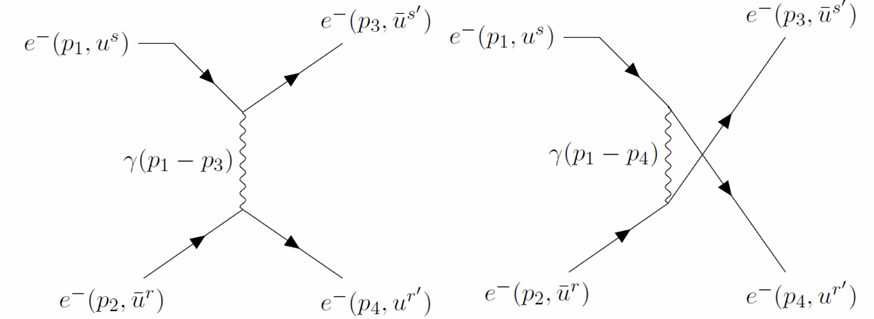
\includegraphics{Moller.png}
  \caption{Diagramás de Feymann de la dispersión Möller}
\end{figure}
\subsubsection{Canal t}
A partir del diagrama, podemos escribir el elemento de matriz:

\begin{equation}
\mathcal{M}_t = (ei\overline{u}_3\gamma^\mu u_1) \frac{ig_{\mu\nu}}{q^2} (ei\overline{v}_4\gamma^\nu u_2) = \frac{e^2}{q^2} [\overline{u}_3\gamma^\mu u_1][\overline{u}_4\gamma^\nu u_2],
\end{equation}

donde el momento del propagador $ q = p_1 - p_3 = \sqrt{t} $. El módulo al cuadrado es

\begin{equation}
\begin{aligned}
|\mathcal{M}_t|^2 &= \frac{e^4}{t^2} [\overline{u}_3\gamma^\mu u_1][\overline{u}_4\gamma^\nu u_2]^* [\overline{u}_3\gamma^\mu u_1]^*[\overline{u}_4\gamma^\nu u_2] \\
&= \frac{e^4}{t^2} [\overline{u}_3\gamma^\mu u_1][\overline{u}_1 \gamma^\rho u_3] [\overline{u}_2 \gamma^\sigma v_4] [\overline{u}_4\gamma^\nu u_2] \\
&= \frac{e^4}{t^2} [\overline{u}_3\gamma^\mu u_1][\overline{u}_1 \gamma^\rho u_3] [\overline{u}_4\gamma^\nu u_1^a][\overline{u}_2 \gamma^\sigma v_4],
\end{aligned}
\end{equation}

donde hemos utilizado la identidad:

\begin{equation}
[\overline{u} \gamma^\rho v]^* = [\overline{u} \gamma^\rho v]^\dagger = v^\dagger \gamma^0 \gamma^\rho \gamma^0 u = v^\dagger (\gamma^0)^2 \gamma^\rho \gamma^0 u = \overline{v} \gamma^\rho u.
\end{equation}
lo cual es válido para espinores $ u $ y $ v $. Dado que las cantidades entre corchetes son números $ C $, podemos tomar sus trazas sin repercusiones:

\begin{equation}
  \begin{aligned}
    |\mathcal{M}_t|^2 = \frac{e^4}{t^2} \text{Tr}[\overline{u}_3\gamma^\nu u_1 \overline{u}_1 \gamma^\nu u_3] \text{Tr}[\overline{u}_2 \gamma^\mu u_4 \overline{u}_4 \gamma^\mu u_2] \\ = \frac{e^4}{t^2} \text{Tr}[u_1 \overline{u}_1 \gamma^\nu u_3 \overline{u}_3 \gamma^\mu] \text{Tr}[u_2 \overline{u}_2 \gamma^\mu u_4 \overline{u}_4 \gamma^\nu].
  \end{aligned}

\end{equation}

Ahora debemos promediar sobre los espines iniciales y sumar sobre los espines finales:

\begin{equation}
|\overline{\mathcal{M}_t}|^2 = \frac{e^4}{4t^2} \text{Tr} \left[ \sum_s u_1^s \overline{u}_1^s \gamma^\nu \sum_{s'} u_3^{s'} \overline{u}_3^{s'} \gamma^\mu \right] \text{Tr} \left[ \sum_r v_2^r \overline{v}_2^r \gamma^\mu \sum_{r'} v_4^{r'} \overline{v}_4^{r'} \gamma^\nu \right],
\end{equation}

usamos las relaciones de completitud para los espinores de Dirac:

\begin{equation}
|\overline{\mathcal{M}_t}|^2 = \frac{e^4}{4t^2} \text{Tr} \left[ (\not{p}_1 - m_e) \gamma^\nu (\not{p}_3 - m_e) \gamma^\mu \right] \text{Tr} \left[ (\not{p}_2 - m_e) \gamma^\mu (\not{p}_4 - m_e) \gamma^\nu \right],
\end{equation}

aquí notaremos que cualquier término que sea lineal en la masa del electrón contendrá un número impar de matrices de Dirac dentro de una traza, la cual se evalúa a cero. Por lo tanto:

\begin{equation}
|\mathcal{M}_t|^2 = \frac{e^4}{4t^2} \left\{ \text{Tr} \left[ \not{p}_1 \not{p}_3 \gamma^\nu \not{p}_3 \gamma^\mu \right] + m_e^2 \, \text{Tr} \left[ \gamma^\nu \gamma^\mu \right] \right\} \left\{ \text{Tr} \left[ \not{p}_2 \not{p}_4 \gamma^\mu \not{p}_4 \gamma^\nu \right] + m_e^2 \, \text{Tr} \left[ \gamma^\mu \gamma^\nu \right] \right\},
\end{equation}

usando las identidades de traza de las matrices de Dirac (Peskin Apéndice 3) esto es

\begin{equation}
|\overline{\mathcal{M}_t}|^2 = \frac{e^4}{4t^2} \left\{ \not{p}_1 \not{p}_3 \, \text{Tr} \left[ \gamma^\nu \gamma^\mu \right] + 4 g_{\mu \nu} m_e^2 \right\} \left\{  p_{2\alpha} p_{4\beta} \, \text{Tr} \left[ \gamma^\mu \gamma^\nu \right] + 4 g_{\mu \nu} m_e^2 \right\},
\end{equation}

las trazas restantes son

\begin{equation}
p_{1\alpha} p_{3\beta} \, \text{Tr} \left[ \gamma^\alpha \gamma^\beta \gamma^\nu \gamma^\mu \right] = 4 p_{1 \alpha} p_{3 \beta} \left( g^{\alpha \beta} g^{\nu \mu} - g^{\alpha \nu} g^{\beta \mu} + g^{\alpha \mu} g^{\beta \nu} \right),
\end{equation}

\begin{equation}
= 4 (p_{1\mu} p_{3\nu} - (p_1 \cdot p_3) g_{\mu\nu} + p_{1\nu} p_{3\mu}),
\end{equation}

\begin{equation}
= 4 p_{2\alpha} p_{4\beta} \left( g^{\alpha \beta} g^{\mu \nu} - g^{\alpha \mu} g^{\beta \nu} + g^{\alpha \nu} g^{\beta \mu} \right),
\end{equation}

\begin{equation}
= 4 (p_{2\mu} p_{4\nu} - (p_2 \cdot p_4) g_{\mu\nu} + p_{2\nu} p_{4\mu}).
\end{equation}

Ahora debemos realizar la multiplicación en la expansión de las matrices. El primer término es la contracción de las dos trazas anteriores, así que usando la notación (1+2+3)(A+B+C), los términos son


las cuales debemos sumar (incluyendo un factor global de $4^2$), observa que el factor de 4 en 2B proviene de $g^{\mu\nu}g_{\mu\nu} = 4$. Notemos las relaciones:

$ 1A = 3C \quad 1C = 3A \quad 2B + 1B + 2A + 2C + 3B = 0, $

así que su suma es

\begin{equation}
4^2 \left[ 2(p_2 \cdot p_1)(p_4 \cdot p_3) + 2(p_4 \cdot p_1)(p_2 \cdot p_3) \right].
\end{equation}

El segundo término (en el elemento de matriz) es la contracción de los dos términos de masa:

\begin{equation}
4^2 g_{\mu\nu} g^{\mu\nu} m_e^4 = 4^2 [4m_e^4].
\end{equation}

Los dos términos restantes son los "términos cruzados":

\begin{equation}
4 (p_{1\mu} p_{3\beta} - (p_1 \cdot p_3) g_{\mu \nu} + p_{1\nu} p_{3\mu})(4g_{\mu \nu} m_e^2) = 4^2 \left[ m_e^2 (p_1 \cdot p_3 - 4p_1 \cdot p_3 + p_1 \cdot p_3) \right]
\end{equation}

\begin{equation}
= 4^2 \left[ -2m_e^2 p_1 \cdot p_3 \right],
\end{equation}

y

\begin{equation}
4 (p_2^\beta p_4^\alpha - (p_2 \cdot p_4) g_{\mu \nu} + p_4^\beta p_2^\alpha)(4g_{\mu \nu} m_e^2) = 4^2 \left[ m_e^2 (p_2 \cdot p_4 - 4(p_2 \cdot p_4) + p_2 \cdot p_4) \right]
\end{equation}

\begin{equation}
= 4^2 \left[ -2m_e^2 p_2 \cdot p_4 \right].
\end{equation}

Reuniendo estos términos, el elemento de matriz es

\begin{equation}
|\overline{\mathcal{M}_t}|^2 = \frac{e^4}{t^2} \left\{ 2(p_2 \cdot p_1)(p_4 \cdot p_3) + 2(p_4 \cdot p_1)(p_2 \cdot p_3) + 4m_e^4 - 2m_e^2(p_1 \cdot p_3) - 2m_e^2(p_2 \cdot p_4) \right\}.
\end{equation}

Nuevamente utilizaremos nuestros invariantes de Mandelstam, observando (en el caso masivo)

\begin{equation}
-2p_1 \cdot p_2 = s - 2m_e^2 = 2ps \cdot p_4,
\end{equation}

\begin{equation}
-2p_1 \cdot p_3 = t - 2m_e^2 = -2p_2 \cdot p_4,
\end{equation}

\begin{equation}
-2p_1 \cdot p_4 = u - 2m_e^2 = -2p_2 \cdot p_3.
\end{equation}

Con estos, el cuadrado del elemento de matriz es

\begin{equation}
|\mathcal{M}_t|^2 = \frac{e^4}{t^2} \left[ (2(p_1 \cdot p_2)(p_4 \cdot p_3) + (2(p_4 \cdot p_1)(p_2 \cdot p_3) + 8m_e^4 - 4m_e^2(p_1 \cdot p_3) - 4m_e^2(p_2 \cdot p_4) \right]
\end{equation}

\begin{equation}
= \frac{e^4}{t^2} \left[ (s - t - m_e^2)^2 + (u - t - m_e^2)^2 + 8m_e^4 + 2m_e^2(t - 2m_e^2) + 2m_e^2(t - 2m_e^2) \right]
\end{equation}

\begin{equation}
= \frac{e^4}{t^2} \left[ s^2 + u^2 + 2sm_e^2 + 2um_e^2 + 4m_e^4 + 2m_e^2(t - 2m_e^2) \right]
\end{equation}

\begin{equation}
= \frac{e^4}{t^2} \left[ s^2 + u^2 + 2sm_e^2 + 2um_e^2 + 4m_e^4 + 4m_e^2t - 8m_e^4 \right]
\end{equation}

\begin{equation}
= \frac{e^4}{t^2} \left[ s^2 + u^2 - 2m_e^2s - 2m_e^2u + 4m_e^2t - 8m_e^4 \right].
\end{equation}

Recuperamos, en el límite ultrarrelativista (i.e., electrón sin masa):

\begin{equation}
|\overline{\mathcal{M}_t}|^2 = 2e^4 \frac{s^2 + u^2}{t^2}.
\end{equation}

\subsubsection{Canal u}

A partir del diagrama, podemos escribir el elemento de matriz:

\begin{equation}
\mathcal{M}_u = (ei\overline{u}_3\gamma^\nu u_1) \frac{ig_{\nu\rho}}{q^2} (ei\overline{u}_4\gamma^\rho u_2) = \frac{e^2}{q^2} [\overline{u}_3\gamma^\nu u_1][\overline{u}_4\gamma^\rho u_2],
\end{equation}

el análisis que sigue se abreviará porque el proceso es casi idéntico al canal t. El cuadrado del módulo del elemento de matriz es

\begin{equation}
|\mathcal{M}_u|^2 = \left( \frac{e^2}{q^2} \right)^2 \left[ [\overline{u}_3\gamma^\nu u_1][\overline{u}_4\gamma^\rho u_2] \right]\left[[\overline{u}_3\gamma_\nu u_1][\overline{u}_2\gamma_\rho u_4]\right]
\end{equation}

\begin{equation}
= \frac{e^4}{q^4} \left[ [\overline{u}_3\gamma^\nu u_1][\overline{u}_4\gamma^\rho u_2]^*[ [\overline{u}_3\gamma_\nu u_1]^*[\overline{u}_2\gamma_\rho u_4] \right]
\end{equation}

\begin{equation}
= \frac{e^4}{q^4} \text{Tr}[u_1\overline{u}_1\gamma^\nu u_4\overline{u}_4\gamma^\rho] \text{Tr}[u_3\overline{u}_3\gamma_\nu u_2\overline{u}_2\gamma_\rho],
\end{equation}

ahora sumamos y promediamos sobre los espines finales e iniciales, y usamos las relaciones de completitud para los espinores de Dirac:

\begin{equation}
|\overline{\mathcal{M}_u}|^2 = \frac{e^4}{4u^2} \text{Tr}[(\not{p}_1 + m)\gamma^\nu (\not{p}_4 + m)\gamma^\rho] \text{Tr}[(\not{p}_2 + m)\gamma^\rho (\not{p}_3 + m)\gamma^\nu]
\end{equation}

\begin{equation}
= \frac{e^4}{4u^2} \left\{ \text{Tr} \left[ \not{p}_1 \not{p}_4 \gamma^\nu \not{p}_4 \gamma^\rho \right] + m^2 \text{Tr}[\gamma^\nu\gamma^\rho] \right\} \left\{ \text{Tr} \left[ \not{p}_2 \not{p}_3 \gamma^\rho \not{p}_3 \gamma^\nu \right] + m^2 \text{Tr}[\gamma^\rho\gamma^\nu] \right\}
\end{equation}

\begin{equation}
= \frac{e^4}{4u^2} \left\{ p_{1\alpha}p_{4\beta} \text{Tr}[\gamma^\alpha\gamma^\beta\gamma^\nu\gamma^\rho] + 4g_{\nu\rho}m^2 \right\} \left\{ p_{2\alpha}p_{3\beta} \text{Tr}[\gamma^\rho\gamma^\nu\gamma^\beta\gamma^\alpha] + 4g_{\rho\nu}m^2 \right\},
\end{equation}

las trazas restantes son

\begin{equation}
p_1^\alpha p_4^\beta \text{Tr}[\gamma_\alpha\gamma_\beta\gamma_\nu\gamma_\rho] = 4p_1^\alpha p_4^\beta (g_{\alpha\nu}g_{\beta\rho} - g_{\alpha\beta}g_{\nu\rho} + g_{\alpha\rho}g_{\beta\nu})
\end{equation}

\begin{equation}
= 4(p_1\cdot p_4)(p_2\cdot p_3) - 4(p_1\cdot p_3)(p_2\cdot p_4),
\end{equation}

\begin{equation}
p_{2\alpha}p_{3\beta} \text{Tr}[\gamma_\rho\gamma_\nu\gamma^\beta\gamma^\alpha] = 4p_{2\alpha}p_{3\beta}\left(g_{\rho\beta}g_{\nu\alpha} - g_{\rho\nu}g_{\beta\alpha} + g_{\rho\alpha}g_{\nu\beta}\right)
\end{equation}

\begin{equation}
= 4(p_2\cdot p_3)(g_{\rho\nu} - (p_2\cdot p_4)) + 4(p_4\cdot p_3),
\end{equation}

que se contraen para dar

\begin{equation}
4^2[2(p_2\cdot p_1)(p_4\cdot p_3) + 2(p_3\cdot p_1)(p_2\cdot p_4)].
\end{equation}

El producto de términos de masa es

\begin{equation}
4^2[4m^4],
\end{equation}

y los términos cruzados son

\begin{equation}
4(p_{1\mu}p_{4\nu} - (p_1\cdot p_4)g_{\mu\nu} + p_{1\nu}p_{4\mu})4m_e^2g_{\mu\nu} = 4^2[-2m_e^2(p_1\cdot p_4)]
\end{equation}

\begin{equation}
4(p_2^\alpha p_3^\beta - (p_2\cdot p_3)g_{\rho\nu} + p_3^\alpha p_2^\beta)4m_e^2g_{\rho\nu} = 4^2[-2m_e^2(p_2\cdot p_3)],
\end{equation}

así que el cuadrado del elemento de matriz es

\begin{equation}
|\overline{\mathcal{M}_u}|^2 = \frac{e^4}{u^2} \left[ 2(p_2 \cdot p_1)(p_4 \cdot p_3) + 2(p_3 \cdot p_1)(p_2 \cdot p_4) + 4m_e^4 - 2m_e^2(p_1 \cdot p_4) - 2m_e^2(p_2 \cdot p_3) \right].
\end{equation}
Escribiendo esto en términos de invariantes de Mandelstam, tenemos

\begin{equation}
|\overline{\mathcal{M}_u}|^2 = \frac{e^4}{u^2} \left\{ 2(p_2 \cdot p_1)(p_3 \cdot p_4) + (-2)(p_3 \cdot p_1)(-2)(p_2 \cdot p_4) + 8m_e^4 - 4m_e^2(p_1 \cdot p_4) - 4m_e^2(p_2 \cdot p_3) \right\},
\end{equation}

\begin{equation}
= \frac{e^4}{u^2} \left\{ [(s - m_e^2)^2 + (t - m_e^2)^2 + 8m_e^4 + 2m_e^2(u - m_e^2) + 2m_e^2(u - m_e^2)] \right\},
\end{equation}

\begin{equation}
|\overline{\mathcal{M}_u}|^2 = \frac{e^4}{u^2} \left[ s^2 + t^2 + 2m_e^2(2u - s - t) + 4m_e^4 \right].
\end{equation}

Recuperamos, en el límite ultrarrelativista (i.e., electrón sin masa):

\begin{equation}
|\overline{\mathcal{M}_u}|^2 = 2e^4 \frac{s^2 + t^2}{u^2}.
\end{equation}

Es interesante notar que podríamos haber encontrado este resultado si hubiéramos hecho las sustituciones $ p_3 \to p_4 $ y $ p_4 \to p_3 $ (nótese que no necesitamos considerar un cambio de signo, ya que no estamos tratando con antipartículas), por lo que los invariantes de Mandelstam se convierten en

\begin{equation}
s = (p_1 + p_2)^2 \rightarrow (p_1 + p_2)^2 = s,
\end{equation}

\begin{equation}
t = (p_3 - p_1)^2 \rightarrow (p_4 - p_1)^2 = u,
\end{equation}

\begin{equation}
u = (p_4 - p_1)^2 \rightarrow (p_3 - p_1)^2 = t.
\end{equation}

\subsubsection{Términos cruzados}
El primer término cruzado es

\begin{equation}
\mathcal{M}_t \mathcal{M}_u^* = \frac{1}{4} \sum_{\text{spins}} \left[ \frac{e^2}{t} [\bar{u}_3 \gamma^\mu u_1] [\bar{u}_4 \gamma_\mu u_2] \right] \left[ \frac{e^2}{u^2} [\bar{u}_4 \gamma^\nu u_1] [\bar{u}_3 \gamma_\nu u_2] \right]
\end{equation}

\begin{equation}
= \frac{e^4}{4tu} \sum_{\text{spins}} [\bar{u}_3 \gamma^\nu u_1] [\bar{u}_4 \gamma_\nu u_2] [\bar{u}_4 \gamma^\mu u_2] [\bar{u}_3 \gamma_\mu u_3]
\end{equation}

\begin{equation}
= \frac{e^4}{4tu} \sum_{\text{spins}} \text{Tr}[\gamma_\nu u_1 \bar{u}_1 \gamma^\mu u_2 \bar{u}_2 \gamma_\mu u_3 \bar{u}_3]
\end{equation}

\begin{equation}
= \frac{e^4}{4tu} \text{Tr}[(\slashed{q}_3 + m) \gamma_\nu (\slashed{p}_4 + m)\gamma^\mu (\slashed{p}_2 + m)\gamma^\nu (\slashed{p}_3 + m)]
\end{equation}

\begin{equation}
= \frac{e^4}{4tu} g_{\mu \rho} g_{\nu \sigma} \text{Tr}[\gamma^\rho (\slashed{p}_4 + m) \gamma^\mu (\slashed{p}_2 + m) \gamma^\sigma (\slashed{p}_3 + m)]
\end{equation}

\begin{equation}
= \frac{e^4}{4tu} g_{\mu \rho} g_{\nu \sigma} \text{Tr}[\gamma^\rho \slashed{p}_4 \gamma^\mu \slashed{p}_2 \gamma^\sigma \slashed{p}_3 ]
\end{equation}

Por el bien de los cálculos, pongamos esto en una forma diferente, usando $ p_1 \to p, \, p_2 \to k,\, p_3 \to p', \, p_4 \to k' $, entonces podemos escribir el término cruzado como

\begin{equation}
\mathcal{M}_t \mathcal{M}_u^* = \frac{e^4}{4st} g_{\mu \alpha} g_{\nu \beta} \text{Tr}[\gamma^\alpha \slashed{k}' \gamma^\mu \slashed{k} \gamma^\beta \slashed{p}'] = \frac{e^4}{4st} g_{\mu \alpha} g_{\nu \beta} \text{Tr}[\gamma^\alpha \slashed{k}' \gamma^\nu \slashed{p} \gamma^\mu \slashed{p}']
\end{equation}

ahora renombramos nuestros índices (intercambiando $\beta$ y $\mu$):

\begin{equation}
\mathcal{M}_t \mathcal{M}_u^* = \frac{e^4}{4tu} g_{\alpha \beta} g_{\mu \nu} \text{Tr}[\gamma^\alpha \gamma^\rho \gamma^\beta \slashed{k}' \slashed{p} \gamma^\nu]
\end{equation}

Nota las siguientes relaciones que se pueden encontrar en el Apéndice A.4 de Schwartz \textit{Quantum Field Theory and the Standard Model}:

\begin{equation}
\gamma^\nu \gamma^\nu = 4
\end{equation}

\begin{equation}
\gamma^\nu \gamma^\mu \gamma^\nu = -2\gamma^\mu
\end{equation}

\begin{equation}
\gamma^\nu \gamma^\mu \gamma^\rho \gamma^\nu = 4g^{\mu \rho}
\end{equation}

\begin{equation}
\gamma^\nu \gamma^\mu \gamma^\rho \gamma^\sigma \gamma^\nu = -2\gamma^\sigma \gamma^\rho \gamma^\mu
\end{equation}

y nota que la cuarta vale para cualquier cantidad impar de matrices gamma entre dos matrices gamma contraídas. Por lo tanto:

\begin{equation}
\mathcal{M}_t \mathcal{M}_u^* = \frac{e^4}{4tu} g_{\alpha \beta} \text{Tr}[\gamma^\alpha \gamma^\rho \gamma^\beta \slashed{k}' \slashed{p} \slashed{p}'] = \frac{e^4}{2tu} g_{\alpha \beta} \text{Tr}[\slashed{k} \gamma^\nu \slashed{p} \gamma^\alpha \gamma^\beta \gamma^\rho]
\end{equation}

\begin{equation}
= \frac{e^4}{2tu} e^2 (p \cdot k')\text{Tr}[\slashed{p} \slashed{k} \gamma^\nu] = e^4 \left( \frac{p_2 \cdot p_4}{p\cdot k'} \right) \text{Tr}[\slashed{p} \cdot \slashed{k}]
\end{equation}

Ahora en términos de los momentos definidos originalmente:

\begin{equation}
\mathcal{M}_t \mathcal{M}_u^* = \frac{-e^8}{stu} (p_1, p_2) (p_3, p_4)
\end{equation}

En términos de los invariantes de Mandelstam esto es

\begin{equation}
\mathcal{M}_t \mathcal{M}_u^* = -8 \frac{e^4}{tu} \left( \frac{s}{2} \right) \left( \frac{s}{2} \right) = -2e^4 \frac{s^2}{tu}.
\end{equation}

En lugar de calcular el otro término cruzado, afirmaré

\begin{equation}
2\text{Re}\{\mathcal{M}_t \mathcal{M}_u^*\} = \mathcal{M}_t \mathcal{M}_u^* + \mathcal{M}_t^* \mathcal{M}_u = 2\text{Re}\{\mathcal{M}_t^* \mathcal{M}_u\},
\end{equation}
así que

\begin{equation}
\mathcal{M}_t \mathcal{M}_u^* + \mathcal{M}_t^* \mathcal{M}_u = -4e^4 \frac{s^2}{tu}.
\end{equation}

\subsubsection{Sección eficaz diferencial}
Para un estado final de dos cuerpos, la sección transversal diferencial está dada por (Peskin eq. 5.12)

\begin{equation}
\frac{d\sigma}{d\Omega} = \frac{1}{2E_{\text{cm}}^2} \frac{|\mathbf{k}|}{16\pi^2 E_{\text{cm}}} |\mathcal{M}|^2.
\end{equation}

En el límite sin masa, en el marco del centro de masa, la sección transversal diferencial se simplifica a

\begin{equation}
\frac{d\sigma}{d\Omega} = \frac{1}{2E_{\text{cm}}} \frac{E_{\text{cm}}/2}{16\pi^2 E_{\text{cm}}} |\mathcal{M}|^2 = \frac{1}{4E_{\text{cm}}} \frac{1}{(4\pi)^2} |\mathcal{M}|^2.
\end{equation}

Usando los elementos de matriz de las secciones sin masa, tenemos

\begin{equation}
\frac{d\sigma}{d\Omega}_t = \frac{1}{4E_{\text{cm}}^2 (4\pi)^2 t^2} e^4 = \left( \frac{\alpha^2}{2s} \right) \frac{s^2 + u^2}{t^2},
\end{equation}

\begin{equation}
\frac{d\sigma}{d\Omega}_u = \frac{1}{4E_{\text{cm}}^2 (4\pi)^2 u^2} e^4 = \left( \frac{\alpha^2}{2s} \right) \frac{s^2 + t^2}{u^2},
\end{equation}

\begin{equation}
\frac{d\sigma}{d\Omega}_{\text{int}} = \frac{1}{4E_{\text{cm}}^2 (4\pi)^2} \frac{e^4 s^2}{tu} = \left( \frac{\alpha^2}{2s} \right) \left( 2 - \frac{s^2}{tu} \right).
\end{equation}

Ahora necesitamos calcular la suma de las secciones transversales diferenciales, pero primero debemos determinar su signo. Como hay fermiones idénticos en el estado final, tenemos que:

\begin{equation}
\mathcal{M} = \mathcal{M}_t - \mathcal{M}_u \quad \Rightarrow \quad |\mathcal{M}|^2 = |\mathcal{M}_t|^2 + |\mathcal{M}_u|^2 - \mathcal{M}_t \mathcal{M}_u^* - \mathcal{M}_t^* \mathcal{M}_u,
\end{equation}

ya que bajo el intercambio de partículas, los sistemas fermiónicos son impares. Entonces

\begin{equation}
\frac{d\sigma}{d\Omega} = \frac{d\sigma}{d\Omega}_t + \frac{d\sigma}{d\Omega}_u + \frac{d\sigma}{d\Omega}_{\text{int}}.
\end{equation}

poniendo nuestros resultados:

\begin{equation}
\frac{d\sigma}{d\Omega} = \frac{\alpha^2}{2s} \left[ \frac{s^2 + u^2}{t^2} + \frac{s^2 + t^2}{u^2} - 2 \left( \frac{t}{u} \right)^2 - 2 \left( \frac{u}{t} \right)^2 \right],
\end{equation}

que se puede escribir como

\begin{equation}
\frac{d\sigma}{d\Omega} = \frac{\alpha^2}{2s} \left( \left( \frac{u}{t} \right)^2 + \left( \frac{t}{u} \right)^2 + \frac{1}{s^2} \right) .
\end{equation}

Si integramos sobre el azimut, adquirimos un factor de $2\pi$, por lo tanto

\begin{equation}
\frac{d\sigma}{d\cos\theta} = \frac{\pi \alpha^2}{s} \left( \left( \frac{u}{t} \right)^2 + \left( \frac{t}{u} \right)^2 + 2 s + \left( \frac{1}{u} \right)^2 + \frac{1}{t^2} \right).
\end{equation}

Investigamos la dependencia angular de la sección transversal diferencial. En el marco del centro de masa, tenemos

$$\begin{aligned}
  p_1 &= (E_{\text{cm}}/2, \mathbf{p}), \\
  p_2 &= (E_{\text{cm}}/2, -\mathbf{p}), \\
  p_3 &= (E_{\text{cm}}/2, \mathbf{k}), \\
  p_4 &= (E_{\text{cm}}/2, -\mathbf{k}).
  \end{aligned}$$

  donde $|\mathbf{p}| = |\mathbf{k}| = E_{\text{cm}}/2$. Usando esto, los invariantes de Mandelstam se pueden escribir como

\begin{equation}
s = 2p_1 \cdot p_2 = E_{\text{cm}}^2
\end{equation}

\begin{equation}
t = -2p_1 \cdot p_3 = -2(p_1^0 p_3^0 - (\mathbf{p} \cdot \mathbf{k}))
= -\frac{E_{\text{cm}}^2}{4} (1 - \cos \theta)
\end{equation}

\begin{equation}
u = -2p_1 \cdot p_4 = -2(p_1^0 p_4^0 - (\mathbf{p} \cdot -\mathbf{k}))
= -\frac{E_{\text{cm}}^2}{4} (1 + \cos \theta)
\end{equation}

Insertando esto en la expresión de la sección transversal diferencial obtenemos

\begin{equation}
\frac{d\sigma}{d\cos \theta} = \frac{\pi \alpha^2}{s} \left[ \left( \frac{-E_{\text{cm}}^2/4}{1 - \cos \theta} \right)^2 + \left( \frac{-E_{\text{cm}}^2/4}{1 + \cos \theta} \right)^2
+ E_{\text{cm}}^4 \left( \frac{1}{-E_{\text{cm}}^2/4 (1 - \cos \theta)} + \frac{1}{-E_{\text{cm}}^2/4 (1 + \cos \theta)} \right)^2 \right]
\end{equation}

la simplificación da como resultado

\begin{equation}
\frac{d\sigma}{d\cos \theta} = \frac{\pi \alpha^2}{s} \left[ \left( \frac{1 + \cos \theta}{1 - \cos \theta}\right)^2 + \left( \frac{1 - \cos \theta}{1 + \cos \theta} \right)^2 + 4 \left( \frac{1}{1 - \cos \theta} + \frac{1}{1 + \cos \theta} \right)^2 \right]
\end{equation}

dejando que nuestro viejo amigo \textsl{MATHEMATICA} maneje el álgebra, obtenemos

\begin{equation}
\frac{d\sigma}{dx} = \frac{\pi \alpha^2}{E_{\text{cm}}^2} \left[ \frac{2 (x^2 + 3)}{(x^2 - 1)^2} \right],
\end{equation}

donde $x = \cos \theta$. Podemos integrar la dependencia angular para ver la dependencia en la energía del centro de masa:

\begin{equation}
\sigma = \int \frac{\pi \alpha^2}{E_{\text{cm}}^2} \left[ \frac{2 (x^2 + 3)}{(x^2 - 1)^2} \right] \, dx = \frac{\pi \alpha^2}{E_{\text{cm}}^2} \left[ x - \frac{8x}{x^2 - 1} \right],
\end{equation}

que diverge en $\pm 1$. Si limitamos la medición a partículas con un ángulo de dispersión mayor que 10°, podemos evaluar la integral numéricamente:

\begin{equation}
\sigma = \int_{\cos(170^\circ)}^{\cos(10^\circ)} \frac{\pi \alpha^2}{E_{\text{cm}}^2} \frac{2 (x^2 + 3)}{(x^2 - 1)^2} \, dx = 1049.05 \frac{\pi \alpha^2}{E_{\text{cm}}^2},
\end{equation}

tener en cuenta que las unidades son GeV$^{-2}$, por lo que tomamos un factor de:

\begin{equation}
\sigma = 1049.05 \frac{0.3894 \, \text{mb}}{1 \, \text{GeV}^{-2}} = \frac{0.06837}{(E_{\text{cm}}/\text{GeV})^2} \, \text{mb}.
\end{equation}

Ahora necesitamos incluir un factor de 1/2 debido a las partículas idénticas en el estado final$^\dagger$, así que

\begin{equation}
\sigma = \frac{0.0342}{(E_{\text{cm}}/\text{GeV})^2} \, \text{mb}.
\end{equation}

Por ejemplo, en haces de electrones colisionando, cada uno con un momento de 4000 GeV (para un \textsl{center-of-mass} de energía de 8000 GeV), la sección transversal total (para la dispersión mayor de 10°) es $\sigma = 5.342 \times 10^{-10}$ mb o 0.534 pb.


\subsection{Dispersión Blhaba}
Hay dos diagramas de Feynman que contribuyen en el proceso:
\begin{figure}
  \centering
  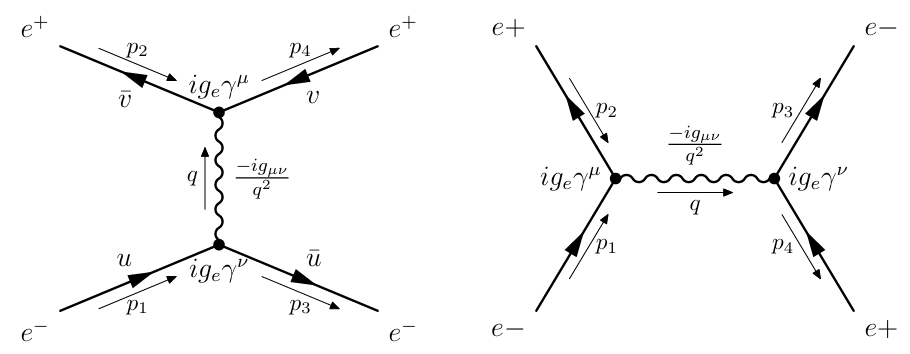
\includegraphics{Bhabha.png}
  \caption{Diagramás de Feymann de la dispersión Bhabha}
\end{figure}
Con amplitudes que denotamos como $ A^{(1)} $ y $ A^{(2)} $ respectivamente. Usando las reglas de Feynman, podemos traducir los diagramas de Feynman en amplitudes:

\begin{equation}
iA^{(1)} = \bar{u}(k')(-ie\gamma^\mu)u(p) \left( \frac{-ig_{\mu\nu}}{q^2} \right) \bar{v}(p')(-ie\gamma^\nu)v(k')
\end{equation}

donde $ q = p - p' = k' - k $.

\begin{equation}
iA^{(2)} = \bar{u}(k')(-ie\gamma^\nu)u(p) \left( \frac{-ig_{\mu\nu}}{q^2} \right) \bar{v}(p')(-ie\gamma^\mu)v(k')
\end{equation}

La amplitud total del proceso es la suma de estos dos:

\begin{equation}
\mathcal{A} = iA^{(1)} + iA^{(2)} 
\end{equation}

Para simplificar las expresiones, introduciremos las variables de Mandelstam:

\begin{equation}
t = (p_1 + p_2)^2 = (p'_1 + p'_2)^2
\end{equation}

\begin{equation}
s = (p_1 - p'_1)^2 = (p_2 - p'_2)^2
\end{equation}

\begin{equation}
u = (p_1 - p'_2)^2 = (p_2 - p'_1)^2
\end{equation}

donde $ p_1 $ y $ p_2 $ son los momentos de las dos partículas iniciales y $ p'_1 $ y $ p'_2 $ son los momentos de las dos partículas finales. Entonces, las amplitudes se pueden escribir como:

\begin{equation}
iA^{(1)} = \left[ \bar{u}(k')\gamma^\nu u(p) \right] \left[ \frac{e^2 g_{\mu\nu}}{s} \right] \left[ \bar{v}(p')\gamma^\mu v(k) \right]
\end{equation}

\begin{equation}
iA^{(2)} = \left[ \bar{u}(k')\gamma^\mu u(p) \right] \left[ \frac{e^2 g_{\mu\nu}}{u} \right] \left[ \bar{v}(p')\gamma^\nu v(k) \right]
\end{equation}

Entonces, el cuadrado de la amplitud es:

\begin{equation}
|\mathcal{A}|^2 = |A^{(1)}|^2 + |A^{(2)}|^2 + 2 \text{Re} \left( A^{(1)} A^{(2)*} \right)
\end{equation}

En la mayoría de los experimentos, los haces de las partículas iniciales no están polarizados y el detector que usamos para estudiar las partículas finales es ciego a la polarización del espín. Entonces, la sección medida es un promedio sobre todas las polarizaciones de los estados final e inicial. Por lo tanto, de hecho, calculamos:

\begin{equation}
  \frac{1}{4} \sum_{\text {spins }}|\mathcal{A}|^2=\frac{1}{4} \sum_{\text {spins }}\left|\mathcal{A}^{(1)}\right|^2+\frac{1}{4} \sum_{\text {spins }}\left|\mathcal{A}^{(2)}\right|^2+\frac{1}{4} \sum_{\text {spins }} \mathcal{A}^{(1)} \mathcal{A}^{(2) *}+\frac{1}{4} \sum_{\text {spins }} \mathcal{A}^{(2)} \mathcal{A}^{(1) *}
  \end{equation}

\subsubsection{Canal t}
Calculamos el canal t para  este proceso: 
\begin{equation}
  \begin{aligned}
  \frac{1}{4} \sum_{\text {spins }}\left|\mathcal{A}^{(1)}\right|^2 & =\frac{1}{4} \sum_{\text {spins }}\left(\frac{i e^2}{s} \eta_{\mu \nu} \bar{v}(k) \gamma^\mu u(p) \bar{u}\left(p^{\prime}\right) \gamma^\nu v\left(k^{\prime}\right)\right)\left(-\frac{i e^2}{s} \eta_{\rho \sigma} \bar{v}\left(k^{\prime}\right) \gamma^\rho u\left(p^{\prime}\right) \bar{u}(p) \gamma^\sigma v(k)\right) \\
  & =\sum_{s p i n s} \frac{e^4}{4 s^2} \eta_{\mu \nu} \eta_{\rho \sigma} \bar{v}(k) \gamma^\mu u(p) \bar{u}\left(p^{\prime}\right) \gamma^\nu v\left(k^{\prime}\right) \bar{v}\left(k^{\prime}\right) \gamma^\rho u\left(p^{\prime}\right) \bar{u}(p) \gamma^\sigma v(k) \\
  & =\sum_{s p i n s} \frac{e^4}{4 s^2} \eta_{\mu \nu} \eta_{\rho \sigma} \bar{v}_a(k) \gamma_{a b}^\mu u_b(p) \bar{u}_c\left(p^{\prime}\right) \gamma_{c d}^\nu v_d\left(k^{\prime}\right) \bar{v}_e\left(k^{\prime}\right) \gamma_{e f}^\rho u_f\left(p^{\prime}\right) \bar{u}_g(p) \gamma_{g h}^\sigma v_h(k) \\
  & =(-1)^{14} \sum_{s p i n s} \frac{e^4}{4 s^2} \eta_{\mu \nu} \eta_{\rho \sigma} \gamma_{a b}^\mu u_b(p) \bar{u}_g(p) \gamma_{g h}^\sigma v_h(k) \bar{v}_a(k) \gamma_{c d}^\nu v_d\left(k^{\prime}\right) \bar{v}_e\left(k^{\prime}\right) \gamma_{e f}^\rho u_f\left(p^{\prime}\right) \bar{u}_c\left(p^{\prime}\right) \\
  & =\frac{e^4}{4 s^2} \eta_{\mu \nu} \eta_{\rho \sigma} \gamma_{a b}^\mu(\not p+m)_{b g} \gamma_{g h}^\sigma(\not k-m)_{h a} \gamma_{c d}^\nu\left(\not k^{\prime}-m\right)_{d e} \gamma_{e f}^\rho\left(\not p^{\prime}+m\right)_{f c} \\
  & =\frac{e^4}{4 s^2} \eta_{\mu \nu} \eta_{\rho \sigma} t r\left(\gamma^\mu(\not p+m) \gamma^\sigma(\not k-m)\right) \operatorname{tr}\left(\gamma^\nu\left(\not k^{\prime}-m\right) \gamma^\rho\left(\not p^{\prime}+m\right)\right) \\
  & =\frac{e^4}{4 s^2} \eta_{\mu \nu} \eta_{\rho \sigma} t r\left((\not k-m) \gamma^\mu(\not p+m) \gamma^\sigma\right) \operatorname{tr}\left(\left(k^{\prime}-m\right) \gamma^\rho\left(\not p^{\prime}+m\right) \gamma^\nu\right)
  \end{aligned}
  \end{equation}

  El factor $(-1)^{14}$ es el resultado de catorce conmutaciones de los campos fermiónicos. En la penúltima línea hemos usado las ecuaciones (3.98) y (3.99). Ahora, computamos cada uno de los trazos por separado, usando la tecnología de trazos que desarrollamos en el capítulo anterior:

\begin{equation}
\text{tr} \left\{ ((k - m) \gamma^\rho (\slashed{p} + m) \gamma^\sigma) \right\} = \text{tr} \left\{ (k^\rho \gamma^\mu + k^\mu \gamma^\rho - m \gamma^\rho)(p_\nu \gamma^\nu + m) \gamma^\sigma \right\}
\end{equation}

\begin{equation}
= \text{tr}(k^\rho \gamma^\mu p_\nu \gamma^\nu \gamma^\sigma + k^\rho m \gamma^\mu \gamma^\sigma - m p_\nu \gamma^\rho \gamma^\nu \gamma^\sigma - m^2 \gamma^\rho \gamma^\sigma)
\end{equation}

\begin{equation}
= k_\rho p_\mu (\gamma^\mu \gamma^\nu \gamma^\nu \gamma^\sigma) + m k_\rho (\gamma^\mu \gamma^\sigma) - m p_\nu (\gamma^\rho \gamma^\nu \gamma^\sigma) - m^2 \text{tr}(\gamma^\rho \gamma^\sigma)
\end{equation}

\begin{equation}
= (4k^\rho p^\sigma - 4(k \cdot p)g^{\rho\sigma} + 4k^\nu p^\rho) - 4m^2 g^{\rho\sigma}
\end{equation}

El siguiente término de traza es:

\begin{equation}
\text{tr} \left\{ ((k' - m) \gamma^\rho (\slashed{p}' + m) \gamma^\sigma) \right\}
\end{equation}

Notamos que este término está conectado al primer traza si realizamos el intercambio: $ k \to k' $ y $ p \to p' $ y $ \mu \to \rho $ y $ \sigma \to \nu $. Así que:

\begin{equation}
\text{tr} \left\{ ((k' - m) \gamma^\rho (\slashed{p}' + m) \gamma^\sigma) \right\} = (4k'^\rho p'^\nu - 4(k' \cdot p')g^{\rho\nu} + 4k^\nu p'^\rho) - 4m^2 g^{\rho\nu}
\end{equation}

Reemplazando los trazos que hemos computado, en la ecuación (6.9), obtenemos:

\begin{equation}
\frac{1}{4} \sum_{\text{spins}} |A^{(1)}|^2 = \frac{e^4}{4s^2} \eta_{\mu\nu} \eta_{\rho\sigma} ((4k'^\rho p'^\nu - 4(k' \cdot p')g^{\rho\nu} + 4k^\nu p'^\rho) - 4m^2 g^{\rho\nu})
\end{equation}

\begin{equation}
((4k^\rho p^\nu - 4(k \cdot p)g^{\rho\sigma} + 4k^\nu p^\rho) - 4m^2 g^{\rho\sigma})
\end{equation}

\begin{equation}
= \frac{4e^4}{s^2} ((k' \cdot p)(k \cdot p) - (k' \cdot k) (p \cdot p) - m^2(k \cdot p))
\end{equation}

\begin{equation}
= \frac{4e^4}{s^2} (m^2 ((p \cdot p) - 4m^2))
\end{equation}

Reuniendo todos los términos, obtenemos:

\begin{equation}
\frac{1}{4} \sum_{\text{spins}} |A^{(1)}|^2 = \frac{8e^4}{s^2} \bigg( (p \cdot p')(k \cdot k') + (p \cdot k)(p' \cdot k') + m^2(k \cdot p') + m^2(k' \cdot p) + 2m^4 \bigg)
\end{equation}

\subsubsection{Canal s}
Procedemos con el cálculo del siguiente término:

\begin{equation}
  \begin{aligned}
  \frac{1}{4} \sum_{\text {spins }}\left|\mathcal{A}^{(2)}\right|^2 & =\frac{1}{4} \sum_{\text {spins }}\left(\frac{i e^2}{t} \eta_{\mu \nu} \bar{u}\left(p^{\prime}\right) \gamma^\mu u(p) \bar{v}(k) \gamma^\nu v\left(k^{\prime}\right)\right)\left(-\frac{i e^2}{t} \eta_{\rho \sigma} \bar{v}\left(k^{\prime}\right) \gamma^\rho v(k) \bar{u}(p) \gamma^\sigma u\left(p^{\prime}\right)\right) \\
  & =\sum_{s p i n s} \frac{e^4}{4 t^2} \eta_{\mu \nu} \eta_{\rho \sigma} \bar{u}\left(p^{\prime}\right) \gamma^\mu u(p) \bar{v}(k) \gamma^\nu v\left(k^{\prime}\right) \bar{v}\left(k^{\prime}\right) \gamma^\rho v(k) \bar{u}(p) \gamma^\sigma u\left(p^{\prime}\right) \\
  & =\sum_{s p i n s} \frac{e^4}{4 t^2} \eta_{\mu \nu} \eta_{\rho \sigma} \bar{u}_a\left(p^{\prime}\right) \gamma_{a b}^\mu u_b(p) \bar{v}_c(k) \gamma_{c d}^\nu v_d\left(k^{\prime}\right) \bar{v}_e\left(k^{\prime}\right) \gamma_{e f}^\rho v_f(k) \bar{u}_g(p) \gamma_{g h}^\sigma u_h\left(p^{\prime}\right) \\
  & =(-1)^{14} \sum_{s p i n s} \frac{e^4}{4 t^2} \eta_{\mu \nu} \eta_{\rho \sigma} \gamma_{a b}^\mu u_b(p) \bar{u}_g(p) \gamma_{g h}^\sigma u_h\left(p^{\prime}\right) \bar{u}_a\left(p^{\prime}\right) \gamma_{c d}^\nu v_d\left(k^{\prime}\right) \bar{v}_e\left(k^{\prime}\right) \gamma_{e f}^\rho v_f(k) \bar{v}_c(k) \\
  & =\frac{e^4}{4 t^2} \eta_{\mu \nu} \eta_{\rho \sigma} \gamma_{a b}^\mu(\not p+m)_{b g} \gamma_{g h}^\sigma\left(\not p^{\prime}+m\right)_{h a} \gamma_{c d}^\nu\left(\not k^{\prime}-m\right)_{d e} \gamma_{e f}^\rho(\not k-m)_{f c} \\
  & =\frac{e^4}{4 t^2} \eta_{\mu \nu} \eta_{\rho \sigma} t r\left(\gamma^\mu(\not p+m) \gamma^\sigma\left(\not p^{\prime}+m\right)\right) t r\left(\gamma^\nu\left(\not k^{\prime}-m\right) \gamma^\rho(\not k-m)\right)
  \end{aligned}
  \end{equation}

El factor $(-1)^{14}$ es el resultado de catorce conmutaciones de los campos fermiónicos. En la penúltima línea hemos usado las ecuaciones (3.98) y (3.99). Vamos a computar ahora cada traza por separado, usando la tecnología de trazas:

\begin{equation}
\text{tr} \left\{ \gamma^\rho (\slashed{p} + m) \gamma^\mu (\slashed{p} + m) \right\} = \text{tr} \left\{ \gamma^\rho \slashed{p} \gamma^\nu \slashed{p} \right\} + m^2 \text{tr}(\gamma^\rho \gamma^\mu)
\end{equation}

\begin{equation}
= 4p^\rho p^\mu + 4m^2 \eta^{\rho\mu}
\end{equation}

Repetimos el mismo procedimiento para el cálculo de la otra traza, obtenemos:

\begin{equation}
\text{tr} \left\{ \gamma^\nu (\slashed{k}' - m) \gamma^\sigma (\slashed{k} - m) \right\} = 4 \left( k'_\rho k_\nu \eta^{\rho\nu} + k_\rho k'_\nu \eta^{\rho\nu} + m^2 \eta^{\rho\nu} \right)
\end{equation}


Usando estas ecuaciones obtenemos: 
\begin{equation}
  \begin{aligned}
  \frac{1}{4} \sum_{s p i n s}\left|\mathcal{A}^{(2)}\right|^2= & \frac{4 e^4}{t^2} \eta_{\mu \nu} \eta_{\rho \sigma}\left(p^\mu p^{\prime \sigma}-\left(p \cdot p^{\prime}\right) \eta^{\mu \sigma}+p^{\prime \mu} p^\sigma+m^2 \eta^{\mu \sigma}\right)\left(k^{\prime \nu} k^\rho-\left(k \cdot k^{\prime}\right) \eta^{\nu \rho}+k^\nu k^{\prime \rho}+m^2 \eta^{\nu \rho}\right) \\
  = & \frac{4 e^4}{t^2} p_\nu p_\rho^{\prime}\left(k^{\prime \nu} k^\rho-\left(k \cdot k^{\prime}\right) \eta^{\nu \rho}+k^\nu k^{\prime \rho}+m^2 \eta^{\nu \rho}\right) \\
  & -\frac{4 e^4}{t^2}\left(p \cdot p^{\prime}\right) \eta_{\nu \rho}\left(k^{\prime \nu} k^\rho-\left(k \cdot k^{\prime}\right) \eta^{\nu \rho}+k^\nu k^{\prime \rho}+m^2 \eta^{\nu \rho}\right) \\
  & +\frac{4 e^4}{t^2} p_\nu^{\prime} p_\rho\left(k^{\prime \nu} k^\rho-\left(k \cdot k^{\prime}\right) \eta^{\nu \rho}+k^\nu k^{\prime \rho}+m^2 \eta^{\nu \rho}\right) \\
  & +\frac{4 m^2 e^4}{t^2} \eta_{\nu \rho}\left(k^{\prime \nu} k^\rho-\left(k \cdot k^{\prime}\right) \eta^{\nu \rho}+k^\nu k^{\prime \rho}+m^2 \eta^{\nu \rho}\right) \\
  = & \frac{4 e^4}{t^2}\left(\left(p \cdot k^{\prime}\right)\left(p^{\prime} \cdot k\right)-\left(k \cdot k^{\prime}\right)\left(p \cdot p^{\prime}\right)+(p \cdot k)\left(p^{\prime} \cdot k^{\prime}\right)+m^2\left(p \cdot p^{\prime}\right)\right) \\
  & -\frac{4 e^4}{t^2}\left(p \cdot p^{\prime}\right)\left(\left(k \cdot k^{\prime}\right)-4\left(k \cdot k^{\prime}\right)+\left(k \cdot k^{\prime}\right)+4 m^2\right) \\
  & +\frac{4 e^4}{t^2}\left(\left(p^{\prime} \cdot k^{\prime}\right)(p \cdot k)-\left(k \cdot k^{\prime}\right)\left(p \cdot p^{\prime}\right)+\left(p^{\prime} \cdot k\right)\left(p \cdot k^{\prime}\right)+m^2\left(p \cdot p^{\prime}\right)\right) \\
  & +\frac{4 m^2 e^4}{t^2}\left(\left(k \cdot k^{\prime}\right)-4\left(k \cdot k^{\prime}\right)+\left(k \cdot k^{\prime}\right)+4 m^2\right) \\
  = & \frac{8 e^4}{t^2}\left(\left(p \cdot k^{\prime}\right)\left(p^{\prime} \cdot k\right)-\left(k \cdot k^{\prime}\right)\left(p \cdot p^{\prime}\right)+(p \cdot k)\left(p^{\prime} \cdot k^{\prime}\right)+m^2\left(p \cdot p^{\prime}\right)+m^2-\left(p \cdot p^{\prime}\right)\right)\left(2 m^2-\left(k \cdot k^{\prime}\right)\right) \\
  = & \frac{8 e^4}{t^2}\left(\left(p \cdot k^{\prime}\right)\left(p^{\prime} \cdot k\right)+(p \cdot k)\left(p^{\prime} \cdot k^{\prime}\right)-m^2\left(p \cdot p^{\prime}\right)-m^2\left(k \cdot k^{\prime}\right)+2 m^4\right)
  \end{aligned}
  \end{equation}

\subsubsection{Términos cruzados}
Los términos $\mathcal{A}^{(1)} \mathcal{A}^{(2)*}$ y $\mathcal{A}^{(2)} \mathcal{A}^{(1)*}$ son ligeramente más complicados. Tenemos:

\begin{equation}
  \begin{aligned}
  \frac{1}{4} \sum_{s p i n s} \mathcal{A}^{(1)} \mathcal{A}^{(2)} & =\frac{1}{4} \sum_{s p i n s}\left(\frac{i e^2}{s} \eta_{\mu \nu} \bar{v}(k) \gamma^\mu u(p) \bar{u}\left(p^{\prime}\right) \gamma^\nu v\left(k^{\prime}\right)\right)\left(-\frac{i e^2}{t} \eta_{\rho \sigma} \bar{v}\left(k^{\prime}\right) \gamma^\sigma v(k) \bar{u}(p) \gamma^\rho u\left(p^{\prime}\right)\right) \\
  & =\frac{e^4}{4 s t} \eta_{\mu \nu} \eta_{\rho \sigma} \sum_{s p i n s} \bar{v}_a(k) \gamma_{a b}^\mu u_b(p) \bar{u}_c\left(p^{\prime}\right) \gamma_{c d}^\nu v_d\left(k^{\prime}\right) \bar{v}_e\left(k^{\prime}\right) \gamma_{e f}^\sigma v_f(k) \bar{u}_g(p) \gamma_{g h}^\rho u_h\left(p^{\prime}\right) \\
  & =(-1)^{15} \frac{e^4}{4 s t} \eta_{\mu \nu} \eta_{\rho \sigma} \sum_{s p i n s} \gamma_{a b}^\mu u_b(p) \bar{u}_g(p) \gamma_{c d}^\nu v_d\left(k^{\prime}\right) \bar{v}_e\left(k^{\prime}\right) \gamma_{e f}^\sigma v_f(k) \bar{v}_a(k) \gamma_{g h}^\rho u_h\left(p^{\prime}\right) \bar{u}_c\left(p^{\prime}\right) \\
  & =-\frac{e^4}{4 s t} \eta_{\mu \nu} \eta_{\rho \sigma} \not k_{f a} \gamma_{a b}^\mu \not p_{b g} \gamma_{g h}^\rho \not p_{h c}^{\prime} \gamma_{c d}^\nu k_{d e}^{\prime} \gamma_{e f}^\sigma \\
  & =-\frac{e^4}{4 s t} \eta_{\mu \nu} \eta_{\rho \sigma} t r\left(\not k \gamma^\mu \not p \gamma^\rho \not p^{\prime} \gamma^\nu \not k^{\prime} \gamma^\sigma\right)
  \end{aligned}
  \end{equation}

Nota que en el paso penúltimo hemos eliminado todos los términos de masa. Para calcular esta traza, utilizaremos el hecho de que:


\begin{equation}
  \gamma^\mu \not p=\gamma^\mu \gamma^\nu p_\nu=p_\nu\left(2 \eta^{\mu \nu}-\gamma^\nu \gamma^\mu\right)=2 p^\mu-\not p \gamma^\mu 
\end{equation}

y

\begin{equation}
  \not p \not p=p_\mu p_\nu \gamma^\mu \gamma^\nu=\frac{1}{2} p_\mu p_\nu\left\{\gamma^\mu, \gamma^\nu\right\}=\frac{1}{2} p_\mu p_\nu 2 \eta^{\mu \nu}=p^2=0
\end{equation}

Luego, usamos la conservación del momento: $ k' = p + k - p' $, para reemplazar $ k' $:

\begin{equation}
  \begin{aligned}
  \frac{1}{4} \sum_{\text {spins }} \mathcal{A}^{(1)} \mathcal{A}^{(2)} & =-\frac{e^4}{4 s t} \eta_{\mu \nu} \eta_{\rho \sigma} \operatorname{tr}\left(\not k \gamma^\mu \not p \gamma^\rho \not p^{\prime} \gamma^\nu \not k^{\prime} \gamma^\sigma\right) \\
  & =-\frac{e^4}{4 s t} \eta_{\mu \nu} \eta_{\rho \sigma} \operatorname{tr}\left(\not k \gamma^\mu \not p \gamma^\rho \not p \gamma^{\prime} \gamma^\nu\left(\not p+\not k-\not p^{\prime}\right) \gamma^\sigma\right)
  \end{aligned}
  \end{equation}

Ahora computamos cada uno de los términos en las trazas separadamente:

\begin{equation}
  \begin{aligned}
  \eta_{\mu \nu} \eta_{\rho \sigma} \operatorname{tr}\left(\not k \gamma^\mu \not p \gamma^\rho \not p^{\prime} \gamma^\nu \not p \gamma^\sigma\right)= & \eta_{\mu \nu} \eta_{\rho \sigma} \operatorname{tr}\left(\not k \gamma^\mu\left(2 p^\rho-\gamma^\rho \not p\right) \not p^{\prime}\left(2 p^\nu-\not p \gamma^\nu\right) \gamma^\sigma\right) \\
  = & 4 \operatorname{tr}\left(\not k \not p \not p^{\prime} \not p\right)-2 \eta_{\mu \nu} \operatorname{tr}\left(\not k \gamma^\mu \not p^{\prime} \not p \gamma^\nu \not p\right)-2 \eta_{\rho \sigma} \operatorname{tr}\left(\not k \not p \gamma^\rho \not p \not p p^{\prime} \gamma^\sigma\right) \\
  & +\eta_{\mu \nu} \eta_{\rho \sigma} \operatorname{tr}\left(\not k \gamma^\mu \gamma^\rho \not p \not p^{\prime} \not p \gamma^\nu \gamma^\sigma\right) \\
  = & 4 \operatorname{tr}\left(\not k \not p\left(2\left(p \cdot p^{\prime}\right)-\not p \not p^{\prime}\right)\right)-2 \eta_{\mu \nu} \operatorname{tr}\left(\not k \gamma^\mu \not p^{\prime}\left(2 p^\nu-\gamma^\nu \not p\right) \not p\right) \\
  & -2 \eta_{\rho \sigma} t r\left(\not k \not p\left(2 p^\rho-\not p \gamma^\rho\right) \not p^{\prime} \gamma^\sigma\right)+\eta_{\mu \nu} \eta_{\rho \sigma} \operatorname{tr}\left(\not k \gamma^\mu \gamma^\rho\left(2\left(p \cdot p^{\prime}\right)-\not p^\prime \not p\right) \not p \gamma^\nu \gamma^\sigma\right)
  \end{aligned}
  \end{equation}

Entonces, usando $ p^2 = m^2 = 0 $:

\begin{equation}
  \begin{aligned}
  \eta_{\mu \nu} \eta_{\rho \sigma} \operatorname{tr}\left(\not k \gamma^\mu \not p \gamma^\rho \not p^{\prime} \gamma^\nu \not p \gamma^\sigma\right)= & 8\left(p \cdot p^{\prime}\right) \operatorname{tr}(\not k \not p)-4 \operatorname{tr}\left(\not k p^2 \not p^{\prime}\right)-4 \operatorname{tr}\left(\not k \not p\not p^{\prime} \not p\right)+2 \eta_{\mu \nu} \operatorname{tr}\left(\not k \gamma^\mu \not p^{\prime} \gamma^\nu p^2\right) \\
  & -4 \operatorname{tr}\left(\not k \not p  \not p^{\prime} \not p\right)+2 \eta_{\rho \sigma} \operatorname{tr}\left(\not k p^2 \gamma^\rho \not p^{\prime} \gamma^\sigma\right)+\eta_{\mu \nu} \eta_{\rho \sigma} 2\left(p \cdot p^{\prime}\right) \operatorname{tr}\left(\not k \gamma^\mu \gamma^\rho \not p \gamma^\nu \gamma^\sigma\right) \\
  & -\eta_{\mu \nu} \eta_{\rho \sigma} \operatorname{tr}\left(\not k \gamma^\mu \gamma^\rho \not p^{\prime} \not p \not p \gamma^\nu \gamma^\sigma\right) \\
  = & 32\left(p \cdot p^{\prime}\right)(k \cdot p)-4 \operatorname{tr}\left(\not  k\not p \not p^{\prime} \not p\right)-4 \operatorname{tr}\left(\not k \not p\not p^{\prime} \not p\right)+2\left(p \cdot p^{\prime}\right) \eta_{\mu \nu} \eta_{\rho \sigma} \operatorname{tr}\left(\not k \gamma^\mu \gamma^\rho \not p \gamma^\nu \gamma^\sigma\right) \\
  = & 32\left(p \cdot p^{\prime}\right)(k \cdot p)-8 \operatorname{tr}\left(\not k\left(2\left(p \cdot p^{\prime}\right)-\not p^{\prime} \not p\right) \not p\right)+2\left(p \cdot p^{\prime}\right) \eta_{\mu \nu} \eta_{\rho \sigma} \operatorname{tr}\left(\not k \gamma^\mu \gamma^\rho \not p \gamma^\nu \gamma^\sigma\right)
  \end{aligned}
  \end{equation}

El último término se convierte en:

\begin{equation}
  \begin{aligned}
  \eta_{\mu \nu} \eta_{\rho \sigma} \operatorname{tr}\left(\not k \gamma^\mu \gamma^\rho \not p \gamma^\nu \gamma^\sigma\right) & =\eta_{\mu \nu} \eta_{\rho \sigma} \operatorname{tr}\left(\left(2 k^\mu-\gamma^\mu \not k\right) \gamma^\rho \not p\left(2 \eta^{\nu \sigma}-\gamma^\sigma \gamma^\nu\right)\right) \\
  & =4 \operatorname{tr}(\not k \not p )-2 \eta_{\rho \sigma} \operatorname{tr}\left(\gamma^\rho \not p \gamma^\sigma \not k\right)-2 \eta_{\mu \rho} \operatorname{tr}\left(\gamma^\mu\not k  \gamma^\rho \not p\right)+4 \eta_{\rho \sigma} \operatorname{tr}\left(\not k \gamma^\rho \not p \gamma^\sigma\right) \\
  & =4 \operatorname{tr}(\not k \not p)-(2+2-4) \eta_{\rho \sigma} \operatorname{tr}\left(\gamma^\rho \not p \gamma^\sigma \not k\right) \\
  & =16 k \cdot p
  \end{aligned}
  \end{equation}

Consecuentemente:

\begin{equation}
  \begin{aligned}
  \eta_{\mu \nu} \eta_{\rho \sigma} \operatorname{tr}\left(\not k \gamma^\mu \not p \gamma^\rho \not p^{\prime} \gamma^\nu \not p \gamma^\sigma\right) & =32\left(p \cdot p^{\prime}\right)(k \cdot p)-16\left(p \cdot p^{\prime}\right) \operatorname{tr}(\not k \not p)+8 \operatorname{tr}\left(\not k \not p^{\prime} \not p\not p \right)+32\left(p \cdot p^{\prime}\right)(k \cdot p) \\
  & =32\left(p \cdot p^{\prime}\right)(k \cdot p)-64\left(p \cdot p^{\prime}\right)(p \cdot k)+32\left(p \cdot p^{\prime}\right)(k \cdot p) \\
  & =0
  \end{aligned}
  \end{equation}

Procedemos con el cálculo del siguiente término de traza, que es relativamente más fácil:

\begin{equation}
  \begin{aligned}
   \eta_{\mu \nu} \eta_{\rho \sigma} \operatorname{tr}\left(\not k \gamma^\mu \not p \gamma^\rho \not p^{\prime} \gamma^\nu \not k \gamma^\sigma\right)&=\eta_{\mu \nu} \eta_{\rho \sigma} \operatorname{tr}\left(\not k \gamma^\mu \not p \gamma^\rho \not p^{\prime} \gamma^\nu\left(2 k^\sigma-\gamma^\sigma \not k\right)\right) \\
  & =2 \eta_{\mu \nu} \operatorname{tr}\left(\not k \gamma^\mu \not p \not k\not p^{\prime} \gamma^\rho\right)-\eta_{\mu \nu} \eta_{\rho \sigma} \operatorname{tr}\left(k \gamma^\mu \not p \gamma^\rho \not p^{\prime} \gamma^\nu \gamma^\sigma \not k\right) \\
  & =2 \eta_{\mu \nu} \operatorname{tr}\left(\left(2 k^\mu-\gamma^\mu \not k\right) \not p \not k \not p^{\prime} \gamma^\nu\right) \\
  & =4 \operatorname{tr}\left(\not p\not k \not p^{\prime} \not k\right)-2 \eta_{\mu \nu} \operatorname{tr}\left(\gamma^\mu \not k\not p \not k \not p^{\prime} \gamma^\nu\right) \\
  & =4 \operatorname{tr}\left(\not p\not k \not p^{\prime} \not k\right)-8 \operatorname{tr}\left(\not k\not p \not k \not p^{\prime}\right) \\
  & =-4 \operatorname{tr}\left(\not p\not k\left(2\left(p^{\prime} \cdot k\right)-\not k \not p^{\prime}\right)\right) \\
  & =-8\left(p^{\prime} \cdot k\right) \operatorname{tr}(\not p \not k)+4 \operatorname{tr}\left(\not p \not k \not k \not p^{\prime}\right) \\
  & =-32\left(p^{\prime} \cdot k\right)(p \cdot k)
  \end{aligned}
  \end{equation}
Continuamos con el siguiente término:

\begin{equation}
  \eta_{\mu \nu} \eta_{\rho \sigma} \operatorname{tr}\left(\not k \gamma^\mu \not p \gamma^\rho \not p^{\prime} \gamma^\nu \not p^{\prime} \gamma^\sigma\right)=\eta_{\mu \nu} \eta_{\rho \sigma} \operatorname{tr}\left(\not p^{\prime} \gamma^\sigma \not k \gamma^\mu \not p \gamma^\rho p^{\prime} \gamma^\nu\right)
  \end{equation}

Podemos calcular esta traza fácilmente si notamos que utilizando la permutación cíclica: $ k \to p' \to p \to k $ y renombrando los índices ficticios se obtiene:

\begin{equation}
  \eta_{\mu \nu} \eta_{\rho \sigma} \operatorname{tr}\left(\not k \gamma^\mu \not p \gamma^\rho \not p^{\prime} \gamma^\nu \not p^{\prime} \gamma^\sigma\right)=-32\left(p \cdot p^{\prime}\right)\left(k \cdot p^{\prime}\right)
  \end{equation}

Por lo tanto:

\begin{equation}
  \begin{aligned}
  \frac{1}{4} \sum_{\text {spins }} \mathcal{A}^{(1)} \mathcal{A}^{(2)} & =-\frac{e^4}{4 s t} \eta_{\mu \nu} \eta_{\rho \sigma} \operatorname{tr}\left(\not k \gamma^\mu \not p  \gamma^\rho \not p^{\prime} \gamma^\nu\left(\not p+\not k-\not p^{\prime}\right) \gamma^\sigma\right) \\
  & =-\frac{e^4}{4 s t}\left(0-32\left(p^{\prime} \cdot k\right)(p \cdot k)+32\left(p \cdot p^{\prime}\right)\left(k \cdot p^{\prime}\right)\right) \\
  & =-\frac{8 e^4}{s t}\left(\left(p \cdot p^{\prime}\right)\left(k \cdot p^{\prime}\right)-\left(p^{\prime} \cdot k\right)(p \cdot k)\right)
  \end{aligned}
  \end{equation}

Calculamos ahora el término $\mathcal{A}^{(2)} \mathcal{A}^{(1)*}$. Tenemos que:

\begin{equation}
  \begin{aligned}
  \frac{1}{4} \sum_{s p i n s} \mathcal{A}^{(2)} \mathcal{A}^{(1) *} & =\frac{1}{4} \sum_{s p i n s}\left(\frac{i e^2}{t} \eta_{\rho \sigma} \bar{u}\left(p^{\prime}\right) \gamma^\rho u(p) \bar{v}(k) \gamma^\sigma v\left(k^{\prime}\right)\right)\left(-\frac{i e^2}{s} \eta_{\mu \nu} \bar{v}\left(k^{\prime}\right) \gamma^\nu u\left(p^{\prime}\right) \bar{u}(p) \gamma^\mu v(k)\right) \\
  & =\frac{e^4}{4 s t} \eta_{\mu \nu} \eta_{\rho \sigma} \sum_{s p i n s} \bar{u}_a\left(p^{\prime}\right) \gamma_{a b}^\rho u_b(p) \bar{v}_c(k) \gamma_{c d}^\sigma v_d\left(k^{\prime}\right) \bar{v}_e\left(k^{\prime}\right) \gamma_{e f}^\nu u_f\left(p^{\prime}\right) \bar{u}_g(p) \gamma_{g h}^\mu u_h(k) \\
  & =(-1)^{15} \frac{e^4}{4 s t} \eta_{\mu \nu} \eta_{\rho \sigma} \sum_{s p i n s} \gamma_{a b}^\rho u_b(p) \bar{u}_g(p) \gamma_{c d}^\sigma v_d\left(k^{\prime}\right) \bar{v}_e\left(k^{\prime}\right) \gamma_{e f}^\nu u_f\left(p^{\prime}\right) \bar{u}_a\left(p^{\prime}\right) \gamma_{g h}^\mu u_h(k) \bar{v}_c(k) \\
  & =-\frac{e^4}{4 s t} \eta_{\mu \nu} \eta_{\rho \sigma} \sum_{s p i n s} \gamma_{a b}^\rho u_b(p) \bar{u}_g(p) \gamma_{g h}^\mu u_h(k) \bar{v}_c(k) \gamma_{c d}^\sigma v_d\left(k^{\prime}\right) \bar{v}_e\left(k^{\prime}\right) \gamma_{e f}^\nu u_f\left(p^{\prime}\right) \bar{u}_a\left(p^{\prime}\right) \\
  & =-\frac{e^4}{4 s t} \eta_{\mu \nu} \eta_{\rho \sigma} t r\left(\gamma^\rho \not p \gamma^\mu \not k \gamma^\sigma \not k^{\prime} \gamma^\nu \not p^{\prime}\right) \\
  & =-\frac{e^4}{4 s t} \eta_{\mu \nu} \eta_{\rho \sigma} t r\left(\not p \gamma^\mu \not k \gamma^\sigma \not k^{\prime} \gamma^\nu \not p^{\prime} \gamma^\rho\right)
  \end{aligned}
  \end{equation}

  Cuando calculamos el termino anterior, calculamos la cantidad: 
  \begin{equation}
    \frac{e^4}{4 s t} \eta_{\mu \nu} \eta_{\rho \sigma} \operatorname{tr}\left(\not k \gamma^\mu \not p \gamma^\rho \not p^{\prime} \gamma^\nu \not k^{\prime} \gamma^\sigma\right)=\frac{8 e^4}{s t}\left(\left(p \cdot p^{\prime}\right)\left(k \cdot p^{\prime}\right)-\left(p^{\prime} \cdot k\right)(p \cdot k)\right)
    \end{equation}
Por lo que ahora basta con cambiar $p\leftrightarrow k$ y $p^{\prime}\leftrightarrow k^{\prime}$ para obtener el resultado final:

    \begin{equation}
      \frac{1}{4} \sum_{\text {spins }} \mathcal{A}^{(2)} \mathcal{A}^{(1) *}=-\frac{8 e^4}{s t}\left(\left(k \cdot k^{\prime}\right)\left(p \cdot k^{\prime}\right)-\left(k^{\prime} \cdot p\right)(k \cdot p)\right)
      \end{equation}

Cogiendo todo lo anterior obtenemos que: 
\begin{equation}
  \begin{aligned}
  \frac{1}{4} \sum_{\text {spins }}|\mathcal{A}|^2= & \frac{1}{4} \sum_{\text {spins }}\left|\mathcal{A}^{(1)}\right|^2+\frac{1}{4} \sum_{\text {spins }}\left|\mathcal{A}^{(2)}\right|^2+\frac{1}{4} \sum_{\text {spins }} \mathcal{A}^{(1)} \mathcal{A}^{(2) *}+\frac{1}{4} \sum_{\text {spins }} \mathcal{A}^{(2)} \mathcal{A}^{(1) *} \\
  = & \frac{8 e^4}{s^2}\left(\left(p \cdot p^{\prime}\right)\left(k \cdot k^{\prime}\right)+\left(p^{\prime} \cdot k\right)\left(p \cdot k^{\prime}\right)+m^2\left(k^{\prime} \cdot p^{\prime}\right)+m^2(k \cdot p)+2 m^4\right) \\
  & +\frac{8 e^4}{t^2}\left(\left(p \cdot k^{\prime}\right)\left(p^{\prime} \cdot k\right)+(p \cdot k)\left(p^{\prime} \cdot k^{\prime}\right)-m^2\left(p \cdot p^{\prime}\right)-m^2\left(k \cdot k^{\prime}\right)+2 m^4\right) \\
  & -\frac{8 e^4}{s t}\left(\left(p \cdot p^{\prime}\right)\left(k \cdot p^{\prime}\right)-\left(p^{\prime} \cdot k\right)(p \cdot k)\right)-\frac{8 e^4}{s t}\left(\left(k \cdot k^{\prime}\right)\left(p \cdot k^{\prime}\right)-\left(k^{\prime} \cdot p\right)(k \cdot p)\right)
  \end{aligned}
  \end{equation}

  Eliminando los terminos que van con la masa obtenemos: 
  \begin{equation}
    \begin{aligned}
    \frac{1}{4} \sum_{\text {spins }}|\mathcal{A}|^2= & \frac{8 e^4}{s^2}\left(\left(p \cdot p^{\prime}\right)\left(k \cdot k^{\prime}\right)+\left(p^{\prime} \cdot k\right)\left(p \cdot k^{\prime}\right)\right)+\frac{8 e^4}{t^2}\left(\left(p \cdot k^{\prime}\right)\left(p^{\prime} \cdot k\right)+(p \cdot k)\left(p^{\prime} \cdot k^{\prime}\right)\right) \\
    & -\frac{8 e^4}{s t}\left(\left(p \cdot p^{\prime}\right)\left(k \cdot p^{\prime}\right)-\left(p^{\prime} \cdot k\right)(p \cdot k)+\left(k \cdot k^{\prime}\right)\left(p \cdot k^{\prime}\right)-\left(k^{\prime} \cdot p\right)(k \cdot p)\right)
    \end{aligned}
    \end{equation}
\subsubsection{Sección eficaz diferencial}
Ahora, movemos el marco de referencia al centro de masa. Establecemos el ángulo entre los electrones del estado inicial y el estado final como $\theta$. Los diferentes cuatro-momentos de las partículas del proceso son:

\begin{equation}
p = (E, \mathbf{p}), \quad k = (E, -\mathbf{p}), \quad p' = (E, \mathbf{p'}), \quad k' = (E, -\mathbf{p'})
\end{equation}

Entonces, establecemos $\mathbf{p}^2 = E^2 - m^2 = E^2$ y calculamos todos los productos internos y las cantidades $t$ y $s$ de la última ecuación del apartado anterior:

\begin{itemize}
    \item $ p \cdot k = E^2 + \mathbf{p}^2 = 2E^2 $
    \item $ p' \cdot k = E^2 + \mathbf{p'} \cdot \mathbf{p} = E^2 + E^2 \cos \theta = E^2 (1 + \cos \theta) $
    \item $ k' \cdot k = E^2 - \mathbf{p'} \cdot \mathbf{p} = E^2 (1 - \cos \theta) $
    \item $ p \cdot p' = E^2 (1 - \cos \theta) $
    \item $ p \cdot k' = E^2 (1 + \cos \theta) $
    \item $ p' \cdot k' = E^2 + \mathbf{p'} \cdot \mathbf{p'} = 2E^2 $
    \item $ t = (p - p')^2 = 2m^2 - 2p \cdot p' = -2E^2(1 - \cos \theta) $
    \item $ s = (p + k)^2 = 4E^2 $
\end{itemize}


\begin{equation}
  \begin{aligned}
  \frac{d \sigma}{d \Omega} & =\frac{e^4}{64 \pi^2 4 E^2}\left(\left(1+\cos ^2 \theta\right)+\frac{2\left(4+(1+\cos \theta)^2\right)}{(1-\cos \theta)^2}\right)+\frac{e^4}{64 \pi^2 4 E^2}\left(\frac{1}{1-\cos \theta}\left(2\left(1-\cos ^2 \theta\right)-4(1+\cos \theta)\right)\right) \\
  & =\frac{e^4}{64 \pi^2 4 E^2}\left(\left(1+\cos ^2 \theta\right)+\frac{2\left(4+(1+\cos \theta)^2\right)}{(1-\cos \theta)^2}+\frac{2\left(1-\cos ^2 \theta\right)}{1-\cos \theta}-\frac{4(1+\cos \theta)}{1-\cos \theta}\right) \\
  & =\frac{e^4}{64 \pi^2 2 E^2}\left(\frac{1}{2}\left(1+\cos ^2 \theta\right)+\frac{1+\cos ^4\left(\frac{\theta}{2}\right)}{\sin ^4\left(\frac{\theta}{2}\right)}+2 \cos ^2\left(\frac{\theta}{2}\right)-\frac{2 \cos ^2\left(\frac{\theta}{2}\right)}{\sin ^2\left(\frac{\theta}{2}\right)}\right) \\
  & =\frac{e^4}{64 \pi^2 2 E^2}\left(\frac{1}{2}\left(1+\cos ^2 \theta\right)+\frac{1+\cos ^4\left(\frac{\theta}{2}\right)}{\sin ^4\left(\frac{\theta}{2}\right)}-\frac{2 \cos ^4\left(\frac{\theta}{2}\right)}{\sin ^2\left(\frac{\theta}{2}\right)}\right)
  \end{aligned}
  \end{equation}
\subsection{Dispersión Compton}
Vamos a considerar ahora un tipo de proceso diferente, la dispersión electrón-fotón que involucra la suma de los dos diagramas de Feynman en la Fig.8.3. Usando las reglas de Feynman de QED, la amplitud invariante del proceso está dada por
$$
\begin{aligned}
i \mathscr{M} & =\bar{u}\left(p_{1}^{\prime}, r^{\prime}\right)\left(-i e \gamma^{\mu}\right) \epsilon_{\mu}^{*}\left(p_{2}^{\prime}, \lambda^{\prime}\right) \frac{i\left(p_{1}+p_{2}+m\right)}{\left(p_{1}+p_{2}\right)^{2}-m^{2}}\left(-i e \gamma^{v}\right) \epsilon_{v}\left(p_{2}, \lambda\right) u\left(p_{1}, r\right) \\
& +\bar{u}\left(p_{1}^{\prime}, r^{\prime}\right)\left(-i e \gamma^{v}\right) \epsilon_{v}\left(p_{2}, \lambda\right) \frac{i\left(\not p_{1}-\not p_{2}^{\prime}+m\right)}{\left(p_{1}-p_{2}^{\prime}\right)^{2}-m^{2}}\left(-i e \gamma^{\mu}\right) \epsilon_{\mu}^{*}\left(p_{2}^{\prime}, \lambda^{\prime}\right) u\left(p_{1}, r\right) \\
& =-i e^{2} \bar{u}\left(p_{1}^{\prime}, r^{\prime}\right) \epsilon_{\mu}^{*}\left(p_{2}^{\prime}, \lambda^{\prime}\right) \epsilon_{v}\left(p_{2}, \lambda\right)\left[\frac{\gamma^{\mu}\left(p_{1}+p_{2}+m\right) \gamma^{v}}{\left(p_{1}+p_{2}\right)^{2}-m^{2}}+\frac{\gamma^{v}\left(p_{1}-\not p_{2}^{\prime}+m\right) \gamma^{\mu}}{\left(p_{1}-p_{2}^{\prime}\right)^{2}-m^{2}}\right] u\left(p_{1}, r\right) \tag{8.29}
\end{aligned}
$$

Nótese que en las dos amplitudes el orden de los espinores es el mismo luego deben sumarse. Esta expresión puede simplificarse, teniendo en cuenta que $p_{1}^{2}=m^{2}$ y $p_{2}^{2}=p_{2}^{\prime 2}=0$ con lo que $\left(p_{1}+p_{2}\right)^{2}-m^{2}=2 p_{1} \cdot p_{2} \mathrm{y}\left(p_{1}-p_{2}^{\prime}\right)-m^{2}=-2 p_{1} \cdot p_{2}^{\prime}$. Por otra parte, en el numerador de los propagadores podemos usar que

\begin{equation*}
\left(p_{1}+m\right) \gamma^{v} u\left(p_{1}\right)=\left(2 p_{1}^{v}-\gamma^{v} p_{1}+\gamma^{v} m\right) u\left(p_{1}\right)=2 p_{1}^{v} u\left(p_{1}\right)-\gamma^{v}\left(p_{1}-m\right) u\left(p_{1}\right)=2 p_{1}^{v} u\left(p_{1}\right) \tag{8.30}
\end{equation*}


\begin{marginfigure}[]
  \includegraphics{}
  \caption[]{Diagramas de Feynman correspondientes a la dispersión Compton electrón-fotón.}
  \labfig{fig:}
\end{marginfigure}

Por tanto,

\begin{equation*}
i \mathscr{M}=-i e^{2} \bar{u}\left(p_{1}^{\prime}, r^{\prime}\right) \epsilon_{\mu}^{*}\left(p_{2}^{\prime}, \lambda^{\prime}\right) \epsilon_{\nu}\left(p_{2}, \lambda\right)\left[\frac{\gamma^{\mu} p_{2} \gamma^{v}+2 \gamma^{\mu} p_{1}^{v}}{2 p_{1} \cdot p_{2}}+\frac{-\gamma^{\mu} p_{2}^{\prime} \gamma^{v}+2 \gamma^{v} p_{1}^{\mu}}{-2 p_{1} \cdot p_{2}^{\prime}}\right] u\left(p_{1}, r\right) \tag{8.31}
\end{equation*}


De forma totalmente análoga al ejemplo anterior, ahora podemos promediar sobre el spin y la polarización de las partículas iniciales y sumar sobre las finales. Para los fermiones usamos el mismo truco, mientras que para los fotones puede demostrarse que

\begin{equation*}
\sum_{\lambda} \epsilon_{\mu}^{*}(p, \lambda) \epsilon_{\nu}(p, \lambda) \rightarrow-\eta_{\mu \nu} \tag{8.32}
\end{equation*}


Esta expresión no es una identidad estricta, pero se puede demostrar que es válida siempre que aparezca en el interior de una amplitud de QED. Utilizando las expresiones anteriores llegamos a

\begin{equation*}
\frac{1}{4} \sum_{\text {spins }}|\mathscr{M}|^{2}=2 e^{4}\left[\frac{p_{1} \cdot p_{2}^{\prime}}{p_{1} \cdot p_{2}}+\frac{p_{1} \cdot p_{2}}{p_{1} \cdot p_{2}^{\prime}}+2 m^{2}\left(\frac{1}{p_{1} \cdot p_{2}}-\frac{1}{p_{1} \cdot p_{2}^{\prime}}\right)+m^{4}\left(\frac{1}{p_{1} \cdot p_{2}}-\frac{1}{p_{1} \cdot p_{2}^{\prime}}\right)^{2}\right] \tag{8.33}
\end{equation*}

que permite calcular la sección eficaz del proceso. En el sistema laboratorio, la sección eficaz diferencial viene dada por la llamada fórmula de Klein-Nishina

\begin{equation*}
\frac{d \sigma_{L A B}}{d \Omega}=\frac{\alpha^{2}}{2 m^{2}}\left(\frac{\omega^{\prime}}{\omega}\right)^{2}\left(\frac{\omega^{\prime}}{\omega}+\frac{\omega}{\omega^{\prime}}-\sin ^{2} \theta\right) \tag{8.34}
\end{equation*}

donde $\omega \mathrm{y} \omega^{\prime}$ son las energías inicial y final del fotón relacionadas por la fórmula de Compton
$$
\frac{1}{\omega^{\prime}}-\frac{1}{\omega}=\frac{1}{m}(1-\cos \theta)
$$
con $\theta$ el ángulo entre la dirección del fotón incidente y el saliente.